\documentclass[11 pt]{article}
\usepackage{graphicx}
\usepackage[export]{adjustbox}
\usepackage{float}
\usepackage{amsmath}
\usepackage{pgfplots}
%\pgfplotsset{compat=1}
\title{EE312 Take-Home Exam 2}
\date{2018\\ March}
\author{Nail Tosun - 2094563 \\ Electric and Electronic Engineering Departmant, METU}
\begin{document}
\maketitle
1)
The reason of $R_{B_2}$ is when output switch high to low  it creates a discharge path for internal capacitances of second transistor.
When $V_{IN}<2.8$ since $Q_2$ transistor will be off and output voltage equal $V_{cc}$. With increasing $V_{in}$ pushes $Q_2$ to saturation region therefore $V_{out}=0.2V$
$$V_{IL}=2.8V, \> V_{IH} = 2.9V, \> V_{OL}=0.2V, \>
V_{OH}=6V$$
\begin{figure}[H]
\centering
\begin{tikzpicture}[
declare function={func(\x)=(\x<=2.8)*(6)+and(\x>2.8,\x<=2.9)*(6-58*\x)+(\x>2.9)*(0.2);}
]
\begin{axis}[xmin=0,xmax=6,samples=21,domain=0:6,
              ymin=0,ymax=6,xlabel=$V_{in}$(Volts),ylabel=$V_{out}$(Volts)
              ]
\addplot[]{func(x)};
\end{axis}
\end{tikzpicture}
\caption{Voltage Transfer Characteristic}
\end{figure}
Region 1: $0<V_{IN}2.8<$
Region 2: $2.8<V_{IN}<2.9$
Region 3: $2.9<V_{IN}6<$
\begin{table}[H]
\centering
\caption{Operation Regions of Transistors and Diodes}
\label{my-label}
\begin{tabular}{llll}
   & Region 1 & Region 2       & Region 3       \\
Q1 & Cut-Off  & Forward Active & Forward Active \\
Q2 & Cut-Off  & Forward Active & Saturation     \\
D1 & On       & On             & On/Off         \\
D2 & Off      & On             & On             \\
D3 & Off      & On             & On             \\
D4 & Off      & On             & On            
\end{tabular}
\end{table}

$$NMH=V_{OH}-V_{IH}= 3.1V$$
$$NML=V_{IL}-V_{OL}= 2.6V$$

For fan-out calculations there are two cases;

Output HIGH case: Since there is $D_1$ diode connected there is no current come from load to driver gate. Therefore we can connect infinitely many load gate.
$$N_H=\infty$$ 

Output LOW case: 
$$I_{C_2}=\frac{V_{cc}-V_{sat}}{12k}+\frac{V_{cc}-V_{D_1}-V_{sat}}{4.7k}$$
$$I_{C_2}=16.76 mA$$
$$max(I_{C_2})=\beta_F \sigma I_{B_1}$$
$$I_{B_1}=\frac{V_{cc}-V_{B_1}}{(1-\rho)R_{B_1}+\rho R_{B_1} \beta_F}$$
$$I_{B_2}=\frac{0.8}{60k} + 36\frac{6-3.6}{((1-\rho)+36\rho )4.7k }$$

$$16.76mA = \sigma(0.013+\frac{18.38}{((1+35\rho )4.7k})\beta_F$$
$$35\rho+1=31.39$$
$$\rho=0.85$$


\begin{figure}[H]
  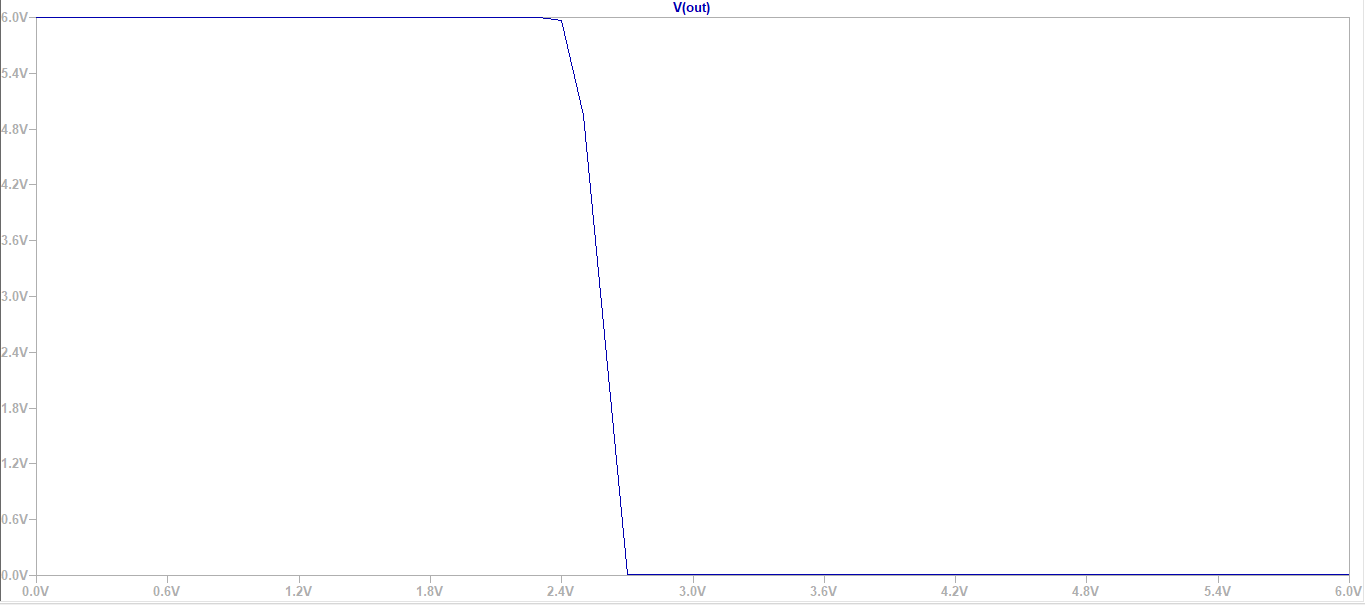
\includegraphics[width=\linewidth]{aa}
  \caption{LTspice simulation results}
  \label{fig:zero}
\end{figure}

2)

\begin{table}[H]
\centering
\caption{Operation Regions of Transistors and Diodes}
\label{my-label}
\begin{tabular}{lllll}
   & Region 1   & Region 2       & Region 3       & Region 4       \\
Q1 & Saturation & Saturation     & Saturation     & Reverse-Active \\
Q2 & Cut-Off    & Forward Active & Saturation
 & Saturation     \\
Q3 & Forward Active & Forward Active    & Saturation-FA     & Cut-Off        \\
Q4 & Cut-Off    & Cut-Off        & Forward-Active & Saturation     \\
D1 & On         & On             & On             & Off            \\
D2 & On         & On             & On             & On            
\end{tabular}
\end{table}




Region 1 : $0 V \leq V_{in} \leq 0.5 V$
$Q_1$ is in saturation region since collector is connected to $Q_2$'s base. Since $V_{CEQ_1}=0.2V+V_{in}$ in this region $Q_2$ is in cut-off region. If $Q_2$ is cut-off region its emitter and collector current is zero. Therefore  $Q_4$'s base is ground therefore $Q_4$ is also cut-off region. $D_1$ diode and $D_2$ diode is open since they are positively bias. For $Q_3$ 
$$V_B=4.3V, \> V_C=5V \> V_E=3.6V$$
Therefore it is forward active region.
$$V_{out}=3.9V$$

Region 2: $0.5 \leq V_{in} < 1.2V$ in this region $Q_2$ is open but since there is enough potential at $Q_4$ base still $Q_4$ is in cut-off region. $V_{out}$ decreases with linearly since t since it collector's($Q_2$) voltage fall :
$$V_{out}=V_C-V_{D_1}-V_{D_2}-0.7$$ $Q_1$ is saturation region. Diodes are open but since $Q_4$ off there is still no current(floating output). $Q_1$ is still saturated. At that point:
$$V_{out}=6-\beta_F I_B-V_{D_1}-V_{D_2}-0.7$$

Region 3: $1.2V \leq V_{in} \leq V_x$ When input hit 1.2V now $Q_4$ will open. $Q_1$ still in saturation. $V_{out}$ drops very quick since $Q_2$ collector voltage drop will faster due to $Q_4$ opening.

Region 4: When $Q_2$ collector voltage drop 2.1 V since $Q_3$ will be off (not enough voltage at BE junction) no current will appear at output. This forces $Q_4$ to saturation and $V{out}$ is fitted to 0.2 V which is output low voltage. 


$V_{OL}=0.2V$, $V_{OH}=3.9V$, $V_{IL}=0.5V$, $V_{IH}=1.4V$
Voltage Transfer Characteristic is following;
\begin{figure}[H]
\centering
\begin{tikzpicture}[
declare function={func(\x)=(\x<=0.5)*(3.9)+and(\x>0.5,\x<=1.2)*(3.9-17/7*\x)+and(\x>1.2,\x<=1.4)*(-10*\x)+(\x>1.4)*(0.2);}
]
\begin{axis}[xmin=0,xmax=6,samples=21,domain=0:6,
              ymin=0,ymax=6,xlabel=$V_{in}$(Volts),ylabel=$V_{out}$(Volts)
              ]
\addplot[]{func(x)};
\end{axis}
\end{tikzpicture}
\caption{Voltage Transfer Characteristic}
\end{figure}

For Fan-out calculation:

1)Output high case

$$V_{out}=V_{IH}+NMH,\> V{IH}=1.4V \> NMH=1V$$
$$V_{out}=2.4V$$
Assuming $Q_3$ is in forward active region. Therefore $I_{C_3}=\beta_F I_{B_3}$

\begin{figure}[H]
  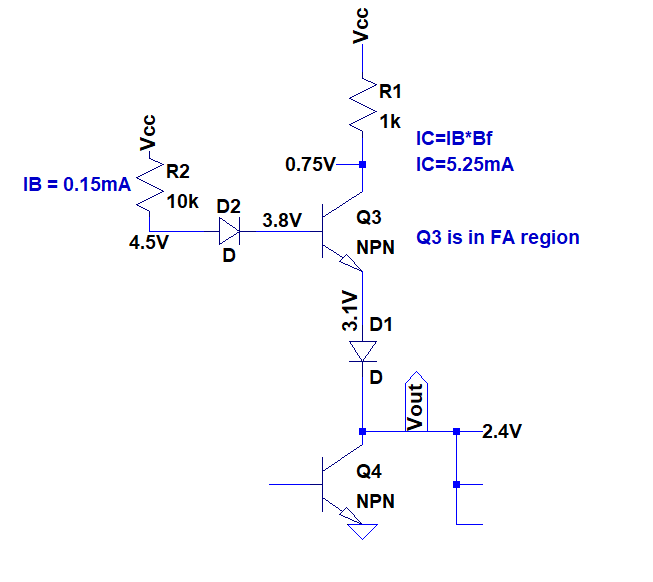
\includegraphics[width=\linewidth]{bb}
  \caption{Assuming $Q_3$ in FA region}
  \label{fig:zero}
\end{figure}

Since $V_{C_3}=0.75$ it is not in FA region. Next assuming is it is in saturation region.

\begin{figure}[H]
  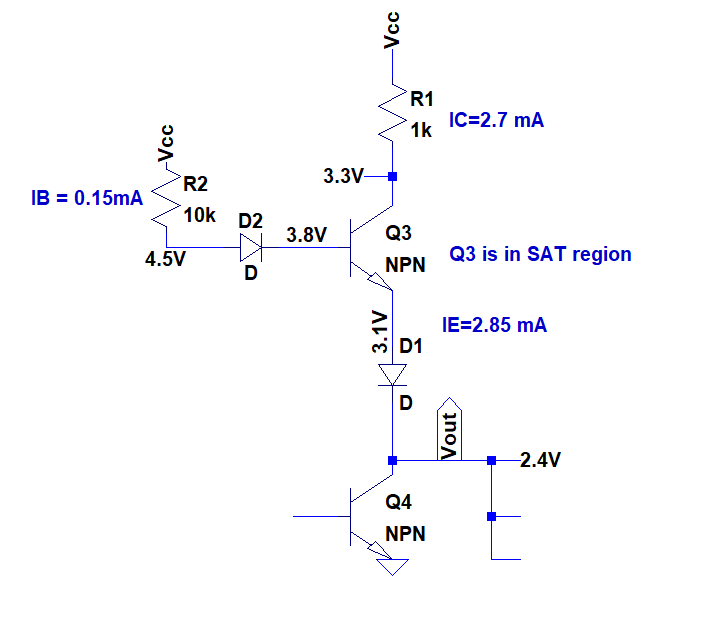
\includegraphics[width=\linewidth]{hk}
  \caption{Assuming $Q_3$ in SAT region}
  \label{fig:zero}
\end{figure}
Now all the voltage values make sense. $I_{OH}=2.85 mA$
\begin{figure}[H]
  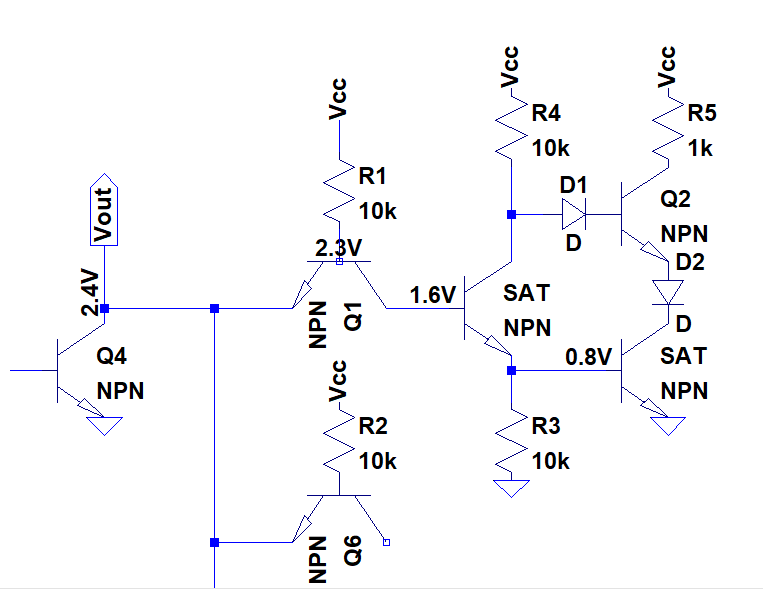
\includegraphics[width=\linewidth]{hi}
  \caption{Maximum fan-out calculation}
  \label{fig:zero}
\end{figure}
$I_{B_1}=0.37mA$ $I_{E_1}=\beta_R I_{B_1}=0.74 mA$
$$\frac{I_{OH}}{I_{E_1}}=3.85$$
$$N=3$$

Output low case;
Driver gate is following:
\begin{figure}[H]
  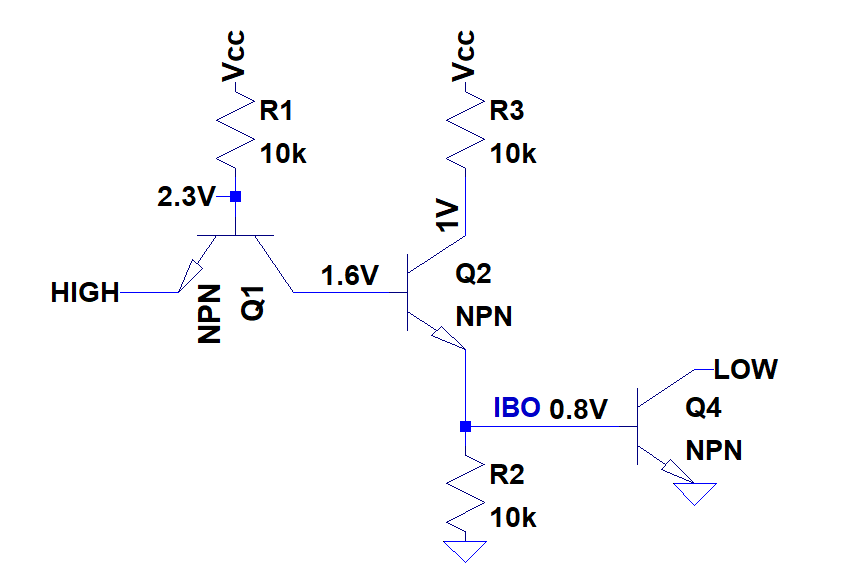
\includegraphics[width=\linewidth]{as}
  \caption{Driver gate}
  \label{fig:zero}
\end{figure}
$$I_{B_1}=0.37mA ,\> I_{C_1}=(\beta_R+1)I_{B_1} I_{C_2}=0.5mA$$ 
$$I_{BO}=(0.5 + 1.11 - 0.08)mA = 1.53 mA $$
$$\sigma_o = \frac{I_{C_{max}}}{\beta_F I_{BO}}$$
$$I_{C_{max}}=42.84 mA$$

\begin{figure}[H]
  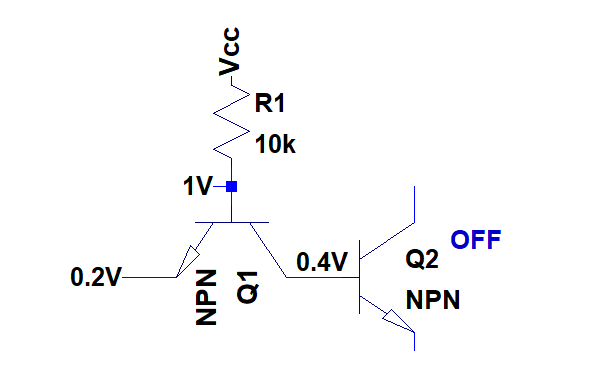
\includegraphics[width=\linewidth]{load}
  \caption{Load gate}
  \label{fig:zero}
\end{figure}

$$N = \frac{42.84}{0.5}=85$$
Maximum fan-out:
3=min(85,3)

Power Consumption:
Output low case:
$P_L=6(0.15)+6(0.5)=3.90mW$
Output high case:
$=6(0.5)=3mW$
$P_{average}=3.45mW$
\end{document}